\documentclass[11pt]{article}


    \usepackage[breakable]{tcolorbox}
    \tcbset{nobeforeafter} % prevents tcolorboxes being placing in paragraphs
    \usepackage{float}
    \floatplacement{figure}{H} % forces figures to be placed at the correct location
    \usepackage{multicol}
	\usepackage[english]{babel}
    \usepackage{tabularx}
    \usepackage{subfigure}
    \usepackage{picture}
    \usepackage{amsmath}
    \usepackage{hyperref}
    \hypersetup{
    colorlinks=true,
    linkcolor=blue,
    filecolor=magenta,      
    urlcolor=cyan,
    }
    \usepackage{graphicx}    
    \usepackage{caption}
    \usepackage{adjustbox} % Used to constrain images to a maximum size 
    \usepackage{xcolor} % Allow colors to be defined
    \usepackage{enumerate} % Needed for markdown enumerations to work
    \usepackage{geometry} % Used to adjust the document margins
    \usepackage{amsmath} % Equations
    \usepackage{amssymb} % Equations
    \definecolor{urlcolor}{rgb}{0,.145,.698}
    \definecolor{linkcolor}{rgb}{.71,0.21,0.01}
    \definecolor{citecolor}{rgb}{.12,.54,.11}
    

    
    % Prevent overflowing lines due to hard-to-break entities
    \sloppy 
    % Setup hyperref package
    \hypersetup{
      breaklinks=true,  % so long urls are correctly broken across lines
      colorlinks=true,
      urlcolor=urlcolor,
      linkcolor=linkcolor,
      citecolor=citecolor,
      }
    % Slightly bigger margins than the latex defaults
    
    \geometry{verbose,tmargin=1in,bmargin=1in,lmargin=0.4in,rmargin=1in}
    \usepackage{fancyhdr}
    \pagestyle{fancy}
    \renewcommand{\footrulewidth}{1pt}
    \rhead{e11921655 Fabian Holzberger \\ e01526208 Jan Ellmenreich}
    \lhead{VU\,184.725\\ High Performance Computing}
    \cfoot{\thepage}
    \setcounter{secnumdepth}{0}
    \setlength\parindent{0pt}

    \usepackage{booktabs}

    \usepackage{listings}
    \usepackage[linesnumbered,ruled,vlined]{algorithm2e}
    \newcommand\mycommfont[1]{\footnotesize\ttfamily\textcolor{blue}{#1}}
    \SetCommentSty{mycommfont}
    \SetKwInput{KwInput}{Input}                % Set the Input
    \SetKwInput{KwOutput}{Output}              % set the Output



\title{Exercise 3.2 Deep learning}
\author{e12045110 Maria de Ronde \\ e12040873  Quentin Andre  \\ e11921655 Fabian Holzberger}
\date{\today}

\begin{document}
\graphicspath{{./pictures/}}
\maketitle
\tableofcontents

%
\section{Datasets}
For exercise 3.2 Deep Learning we decided to apply deep learning on image classification. The data sets that we will use are CIFAR-10 \footnote{\url{https://www.cs.toronto.edu/~kriz/cifar.html}} and Tiny-ImagenNet  \footnote{\url{http://cs231n.stanford.edu/tiny-imagenet-200.zip}}. With these two datasets we have variation in the number of classes represented in the data. This  enables us to explore the difference in performance when the number of classes increase. In sections \ref{Sec_Cifar-10} and \ref{Sec_ImageNet} both datasets are described in more detail. The pictures also differ in input size.\\
We used Python as our programming language and implemented the deep learning using Tensor Flow. 


\subsection{CIFAR-10}\label{Sec_Cifar-10}
CIFAR-10 is a dataset which consists of $60.000$ images, of which $50.000$ training images and $10.000$ test images. Each image has $32\times32$ colored pixels.
There are $10$ different classes (airplane, automobile, bird, cat, deer, dog, frog, horse, ship and truck) each class has exactly $5.000$ images in the training data and $1.000$ images in the test data. Each image only belongs to one class. There are no multi-label images. 

\subsection{Tiny ImageNet}\label{Sec_ImageNet}
Tiny ImageNet is a dataset containing of $100.000$ training images, divided in $200$ different classes. There are $500$ images per class in the training data. Next for the training data there are $10.000$ testing and $10.000$ validation images as well. Each picture has $64\times64$ pixels. The images in the test-set are not labelled and therefore we will not make use of them. To load the data some code from Github \footnote{\url{https://github.com/rmccorm4/Tiny-Imagenet-200}} was used. 

\section{Traditional classifiers}

In order to have a baseline for our deep classifier some traditional classifiers have been executed. The following traditional classifiers have been trained:

\begin{enumerate}
\item{%
\textbf{Multinomial Naive Bayes}: 
\texttt{alpha = 1.0}, \texttt{fit\_prior= True}, \texttt{class\_prior= None}
}
\item{%
\textbf{Random forest}: 
\texttt{n\_estimators = 100}, \texttt{criterion='gini'}, \texttt{max\_depth=None}, \texttt{min\_samples\_split=2}, \texttt{min\_samples\_leaf=1}, \texttt{min\_weight\_fraction\_leaf=0.0}, \texttt{max\_features='auto'}, \texttt{max\_leaf\_nodes = None}, \texttt{min\_impurity\_decrease=0.0}, \texttt{min\_impurity\_split=None}, \texttt{bootstrap=True}, \texttt{oob\_score=False}, \texttt{n\_jobs=None}, \texttt{random\_state=None}, \texttt{verbose=0}, \texttt{warm\_start=False}, \texttt{class\_weight=None}, \texttt{cc\_alpha=0.0}, \texttt{max\_samples=None}
}
\item{%
\textbf{Single layer perceptron}:  
\texttt{penalty=None}, \texttt{alpha=0.0001}, \texttt{l1\_ratio=0.15}, \texttt{fit\_intercept=True}, \texttt{max\_iter=1000}, \texttt{tol=0.001}, \texttt{shuffle=True}, \texttt{verbose=0}, \texttt{eta0=1.0}, \texttt{n\_jobs=None}, \texttt{random\_state=0}, \texttt{early\_stopping=False}, \texttt{validation\_fraction=0.1}, \texttt{n\_iter\_no\_change=5}, \texttt{class\_weight=None}, \texttt{warm\_start=False}
}
\item{%
\textbf{Multi layer perceptron}: 
2 Relu activation layers 256, 1 softmax activation 10  \texttt{epochs=15}, \texttt{batch\_size=32}, \texttt{verbose=0}
}
\end{enumerate}

Before we could train the traditional classifiers, we extracted features from our images. We performed two type of feature extraction. 

\begin{enumerate}
\item{Color histogram}
\item{SIFT}
\end{enumerate}

\subsection{Color histograms}
Color histograms is one of the simplest feature extraction method for images. It counts the frequency of pixels with a certain color. The bins are based on the RGB coding, each pixel has a value for red, green and blue between 0 and 255. Color histograms do not take spatial information into account. All spatial information gets lost during this feature extraction. In Figure\ref{Example-pictures} an example picture with the corresponding color histogram for both datasets is given.\\
%
\begin{figure}[H]
\begin{minipage}[c]{0.4\textwidth}
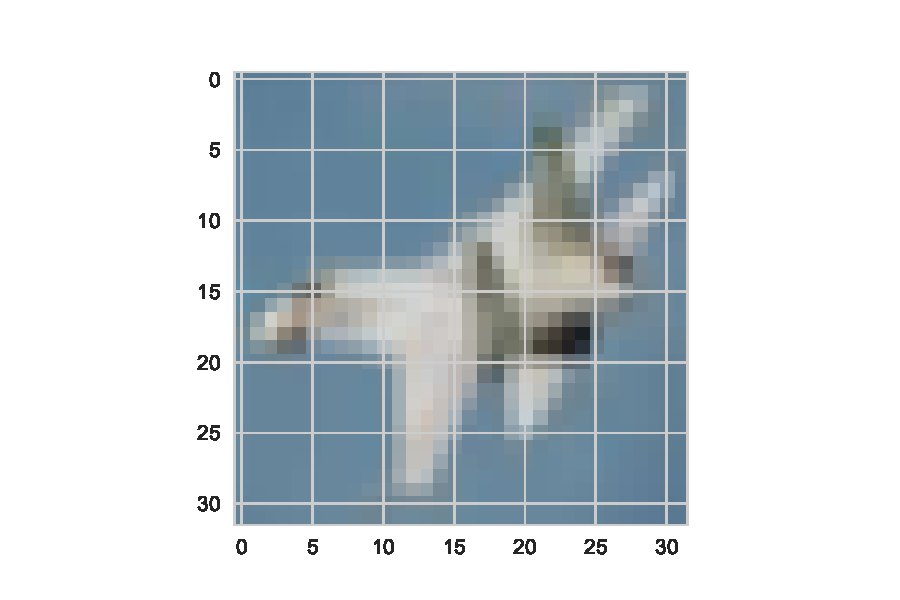
\includegraphics[width=1\linewidth]{figures/Example_picture_Cifar.pdf}
\end{minipage}
\begin{minipage}[d]{0.6\textwidth}
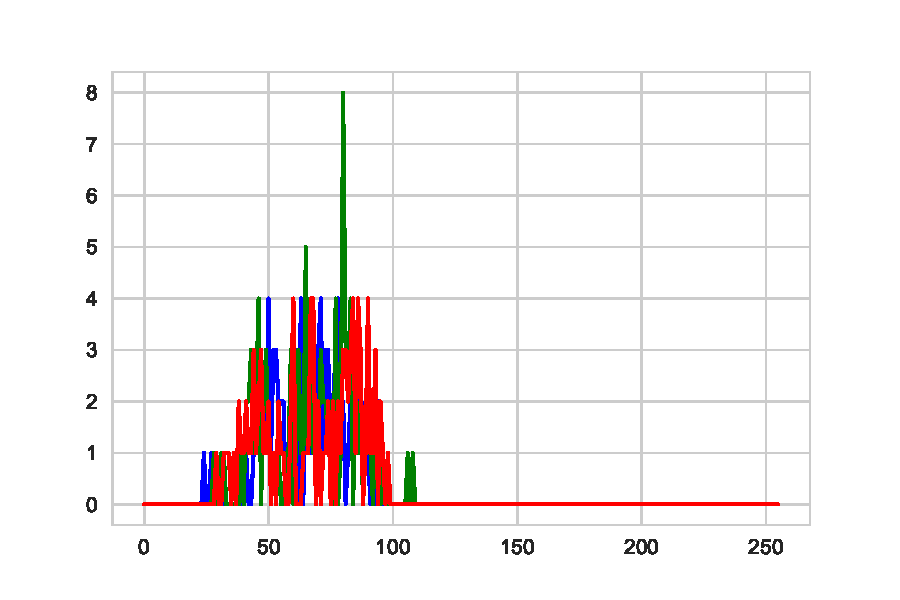
\includegraphics[width=1\linewidth]{figures/Example_picture_Cifar_hist.pdf}
\end{minipage}
\begin{minipage}[c]{0.4\textwidth}
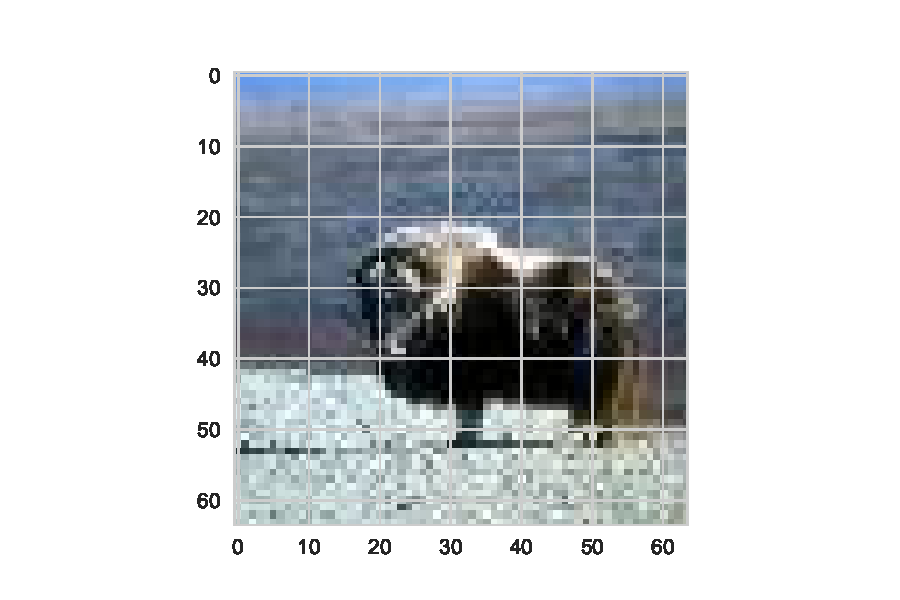
\includegraphics[width=1\linewidth]{figures/Example_picture_Tiny_Image.pdf}
\end{minipage}
\begin{minipage}[d]{0.6\textwidth}
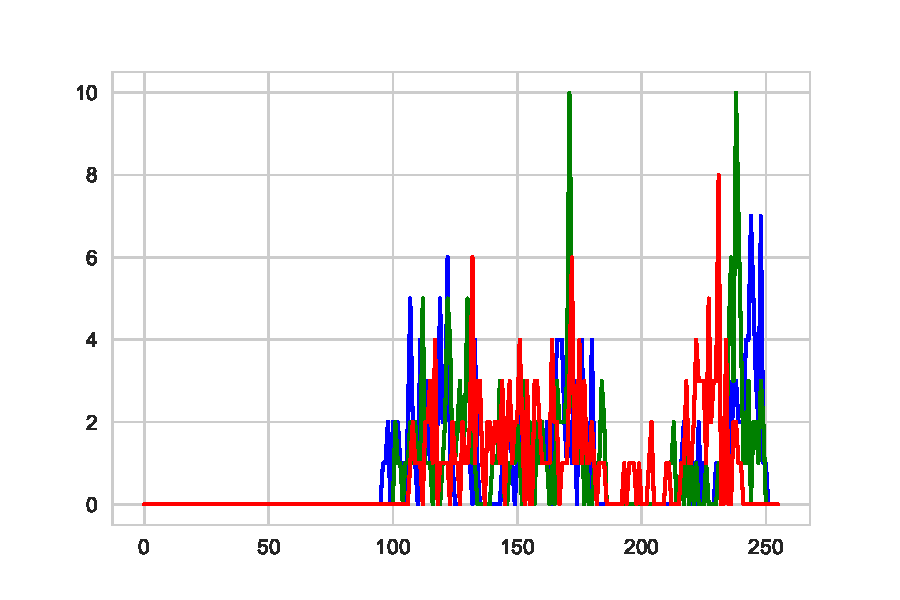
\includegraphics[width=1\linewidth]{figures/Example_picture_Tiny_Image_hist.pdf}
\end{minipage}
\caption{Top: Example picture and color histigram of Cifar dataset. Down: Example picture and color histigram of Tiny Imagenet dataset}
\label{Example-pictures}
\end{figure}

We created 4 different datasets using color hisograms, two based on one dimensional histograms (one with 256 bins per channel and one with 64 bins per channel), one on two dimensional histograms (16 bins per channel) and one of 3 dimensional histograms (8 bins per channel). This is based on the example shown in simple-image-feature-extraction 
\footnote{\url{https://tuwel.tuwien.ac.at/course/view.php?id=35929}}. In order to create the color histograms we used the package OpenCV. 

\subsection{Sift back of visual words}

First the images are converted into grey scale images. With use of SIFT the key-points and descriptors are detected. K-means-clustering is applied to find 20 clusters in the detected descriptors. \\
Finally vectors with the visual words are created and vectorized in a histogram (frequency of visual words). The histogram is scaled to a standard normal distribution before running the classifiers.   
\subsection{Results}
In Figure \ref{Accuracy_Cifar} and \ref{Accuracy_Tiny_Image} the accuracy for the different base classifiers can be found for the Cifar-10 and Tiny image dataset respectively. 
It can be seen that the random forest out performs all classifiers with the color histogram features, the best performance was obtained using the 2-d color histograms.\\
%
Accuracy of BOW
%
The confusion matrices shown in Figure \ref{CV_Matrices_Cifar_color_hist} are based on the 2-d feature color histograms as this gave the best results. The confusion matrix of the single-layer-perceptron shows pretty much a random classifier. Furthermore it can be seen that trucks are often classified as cars and birds are often classified as ship\\. 
The confusion matrix of the Naive Bayes, Random Forest and multi-layer-perceptron show similar results. They show that airplanes, ships and trucks are predicted best even though airplanes and ships are also often confused. It can also be seen that the different animals get confused.

\begin{figure}[H]
\begin{minipage}[c]{0.5\textwidth}
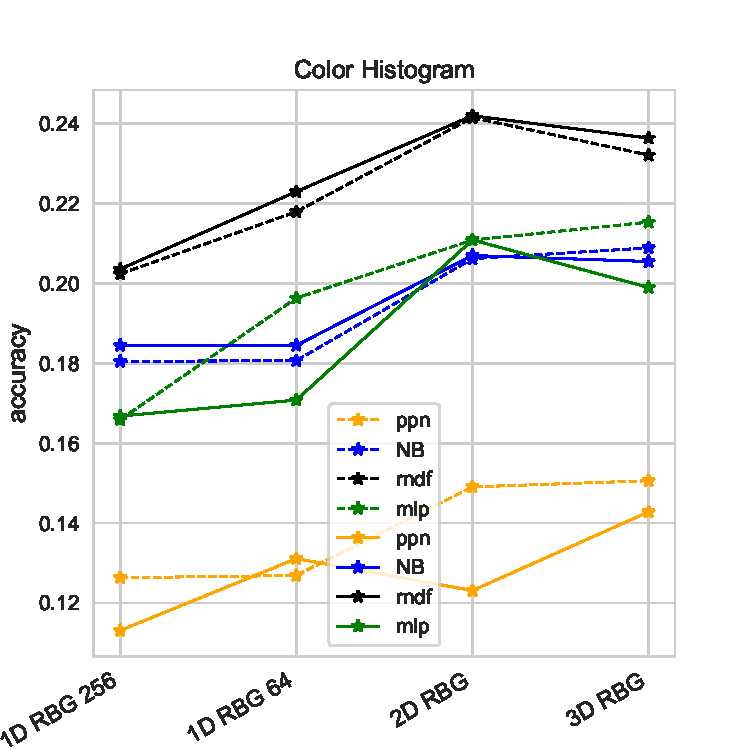
\includegraphics[width=1\linewidth]{figures/Cifar/Accuracy_color_hist.pdf}
\end{minipage}
\begin{minipage}[c]{0.5\textwidth}
\includegraphics[width=1\linewidth]{figures/Cifar/Accuracy_BOW.pdf}
\end{minipage}
\caption{Accuracy Cifar-10}
\label{Accuracy_Cifar}
\end{figure}



\begin{figure}[H]
\begin{minipage}[c]{0.5\textwidth}
\includegraphics[width=1\linewidth]{figures/Cifar/CM__NB_color_hist.pdf}
\end{minipage}
\begin{minipage}[c]{0.5\textwidth}
\includegraphics[width=1\linewidth]{figures/Cifar/CM__Rndf_color_hist.pdf}
\end{minipage}
\begin{minipage}[c]{0.5\textwidth}
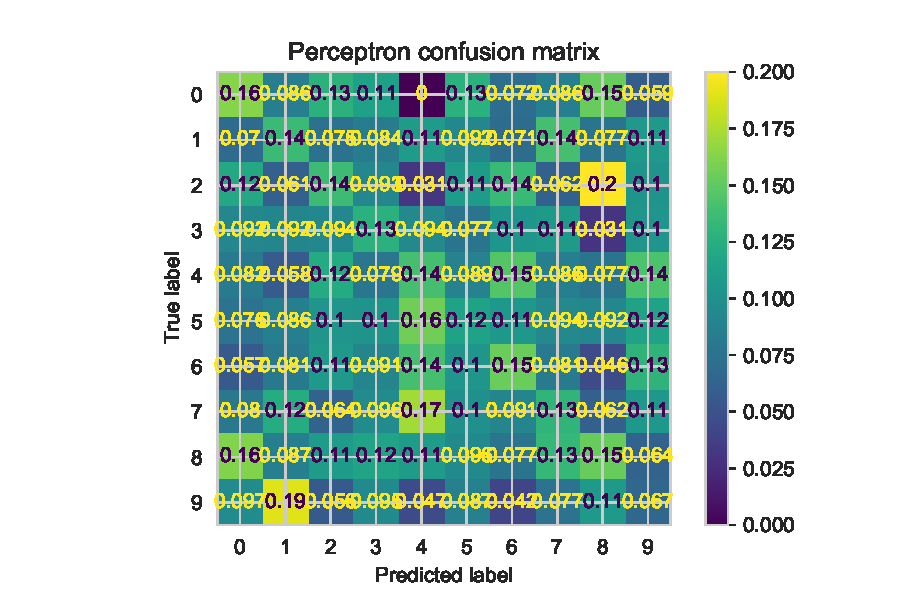
\includegraphics[width=1\linewidth]{figures/Cifar/CM__ppn_color_hist.pdf}
\end{minipage}
\begin{minipage}[c]{0.5\textwidth}

\includegraphics[width=1\linewidth]{figures/Cifar/CM__MLP_color_hist.pdf}
\end{minipage}
\caption{Confusion matrices color histogram Cifar-10: 1. Naive Bayes 2. Random forest 3. Single-layer-perceptron 4. Multi-layer-perceptron}
\label{CV_Matrices_Cifar_color_hist}
\end{figure}


\begin{figure}[H]
\begin{minipage}[c]{0.5\textwidth}
\includegraphics[width=1\linewidth]{figures/Cifar/CM__NB_BOW.pdf}
\end{minipage}
\begin{minipage}[c]{0.5\textwidth}
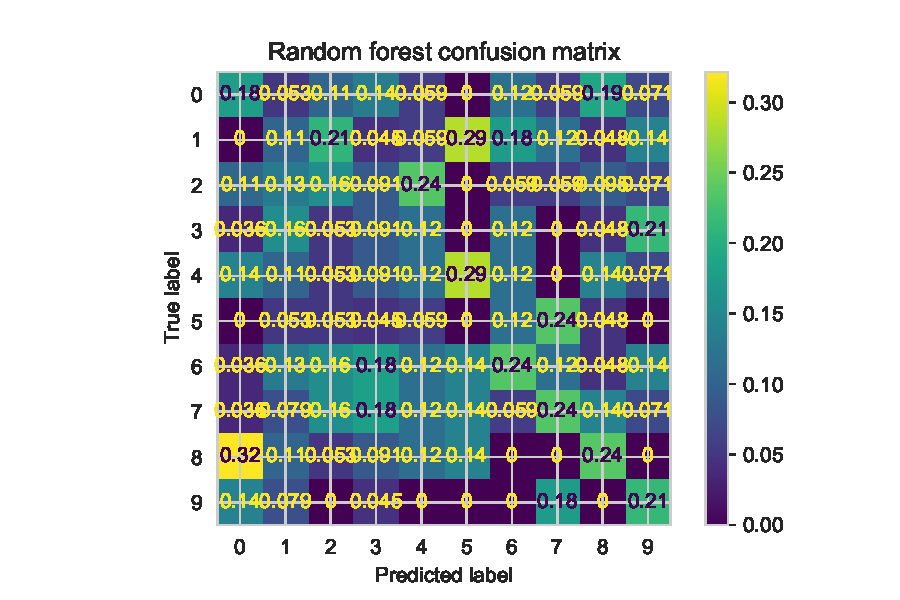
\includegraphics[width=1\linewidth]{figures/Cifar/CM__Rndf_BOW.pdf}
\end{minipage}
\begin{minipage}[c]{0.5\textwidth}
\includegraphics[width=1\linewidth]{figures/Cifar/CM__ppn_BOW.pdf}
\end{minipage}
\begin{minipage}[c]{0.5\textwidth}

\includegraphics[width=1\linewidth]{figures/Cifar/CM__MLP_BOW.pdf}
\end{minipage}
\caption{Confusion matrices bag of words Cifar-10: 1. Naive Bayes 2. Random forest 3. Single-layer-perceptron 4. Multi-layer-perceptron}
\label{CV_Matrices_Cifar_BOW}
\end{figure}

\begin{figure}[H]
\begin{minipage}[c]{0.3\textwidth}
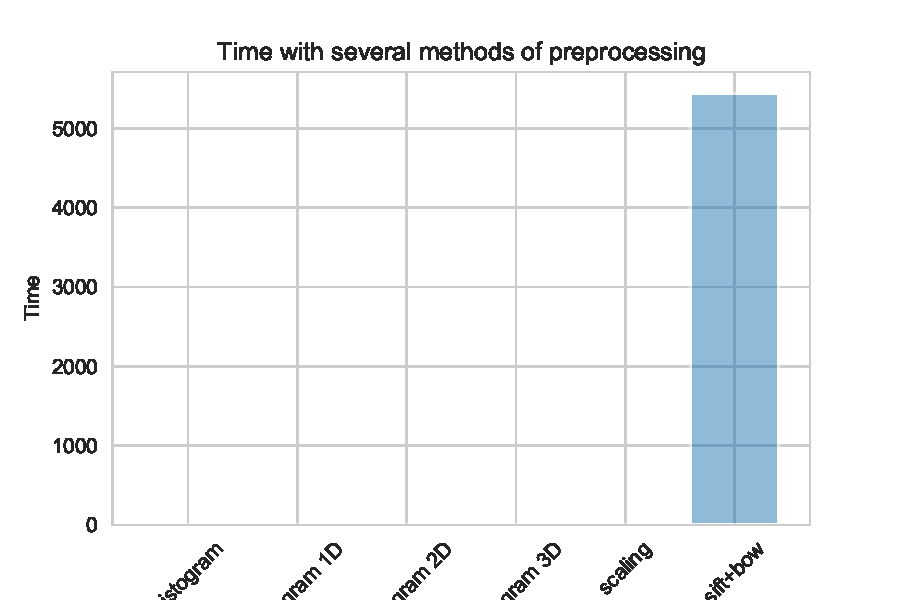
\includegraphics[width=1\linewidth]{figures/Cifar/time_prepro.pdf}
\end{minipage}
\begin{minipage}[c]{0.3\textwidth}
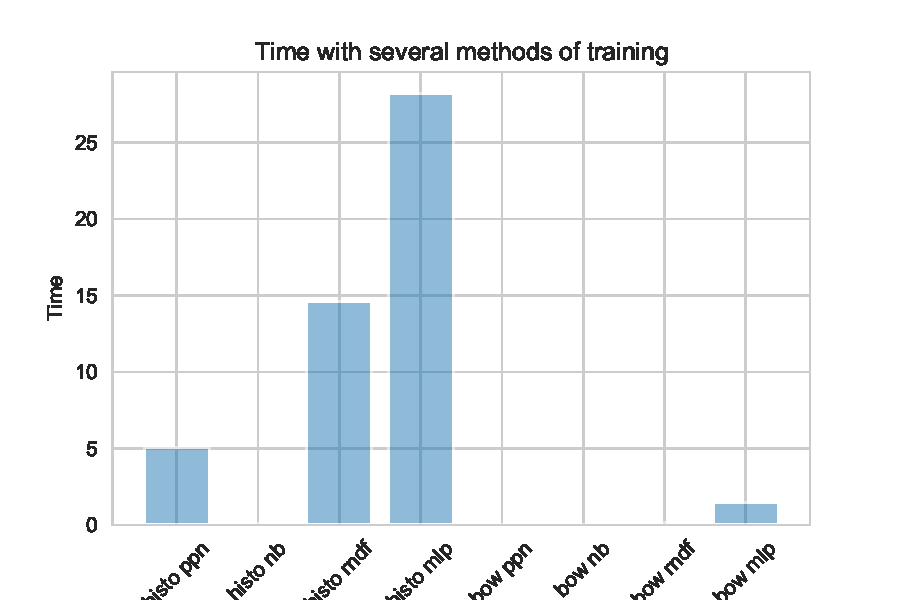
\includegraphics[width=1\linewidth]{figures/Cifar/time_training.pdf}
\end{minipage}
\begin{minipage}[c]{0.3\textwidth}
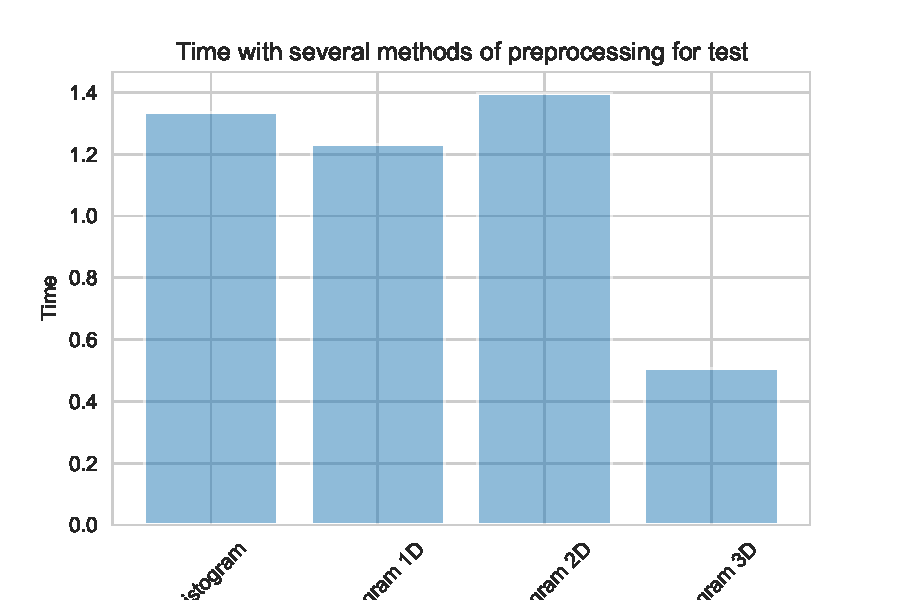
\includegraphics[width=1\linewidth]{figures/Cifar/time_training_test.pdf}
\end{minipage}
\caption{Comparison of time required for different feature extractions and training of models}
\label{Cifar_time_comparison}
\end{figure}


\begin{comment}
%%%%%%%%%%%%%%%%%%%%%%%%%%%%%%%%%%%%%%%%%%%%%%%%%%%%%%%%%%%%%%

\begin{figure}[h]
\begin{minipage}[c]{0.5\textwidth}
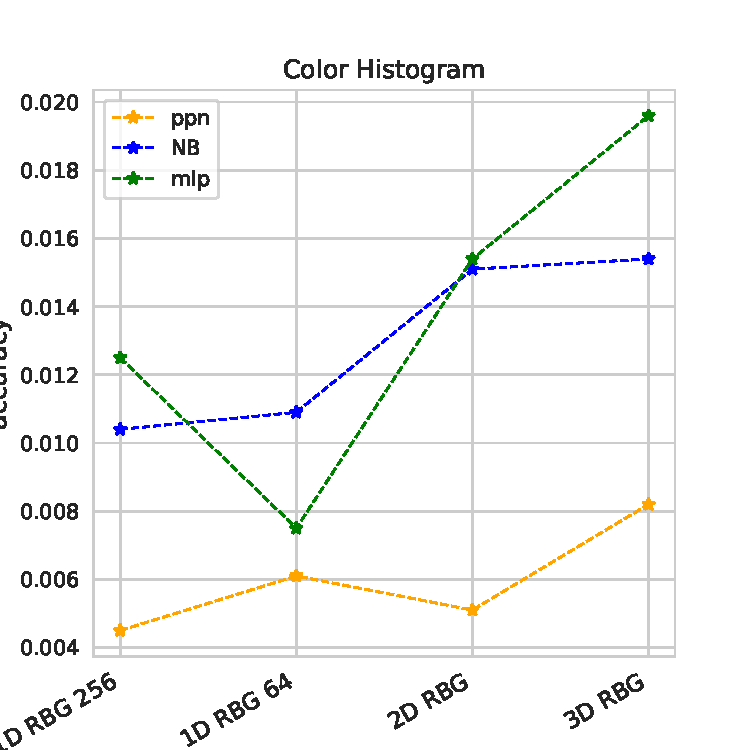
\includegraphics[width=1\linewidth]{figures/Tiny_Image/Accuracy_color_hist.pdf}
\end{minipage}
\begin{minipage}[c]{0.5\textwidth}
\includegraphics[width=1\linewidth]{figures/Tiny_Image/Accuracy_BOW.pdf}
\end{minipage}
\caption{Accuracy Tiny-Image}
\label{Accuracy_Tiny_Image}
\end{figure}
%
\begin{figure}[h]
\begin{minipage}[c]{0.5\textwidth}
\includegraphics[width=1\linewidth]{figures/Tiny_Image/CM__NB_color_hist.pdf}
\end{minipage}
\begin{minipage}[c]{0.5\textwidth}
\includegraphics[width=1\linewidth]{figures/Tiny_Image/CM__Rndf_color_hist.pdf}
\end{minipage}
\begin{minipage}[c]{0.5\textwidth}
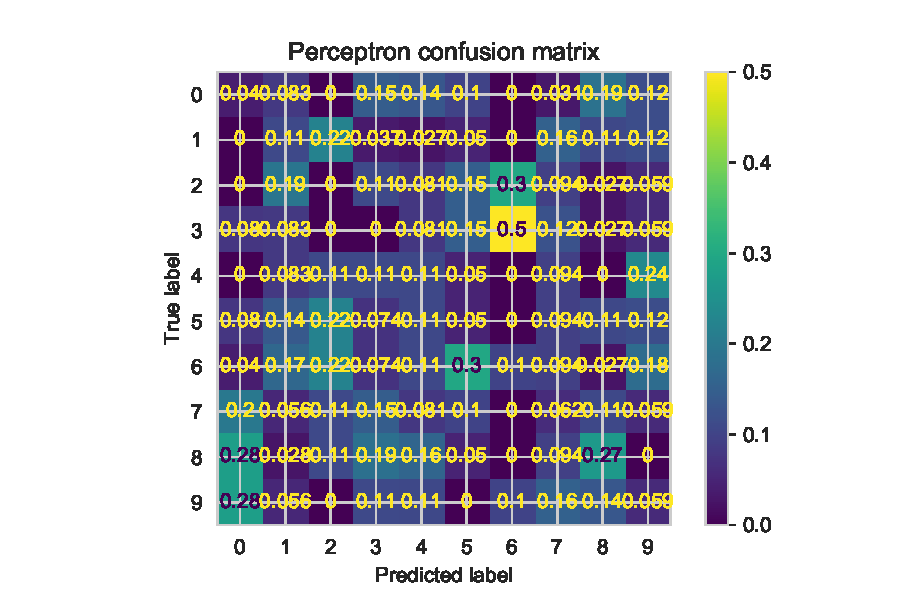
\includegraphics[width=1\linewidth]{figures/Tiny_Image/CM__ppn_color_hist.pdf}
\end{minipage}
\begin{minipage}[c]{0.5\textwidth}

\includegraphics[width=1\linewidth]{figures/Tiny_Image/CM__MLP_color_hist.pdf}
\end{minipage}
\caption{Convusion matrices color histogram 1. Naive Bayes 2. Random forest 3. Single layer Perceptron 4. Multi layer perceptron}
\label{CV_Matrices_Tiny_Image_color_hist}
\end{figure}


\begin{figure}[h]
\begin{minipage}[c]{0.5\textwidth}
\includegraphics[width=1\linewidth]{figures/Tiny_Image/CM__NB_BOW.pdf}
\end{minipage}
\begin{minipage}[c]{0.5\textwidth}
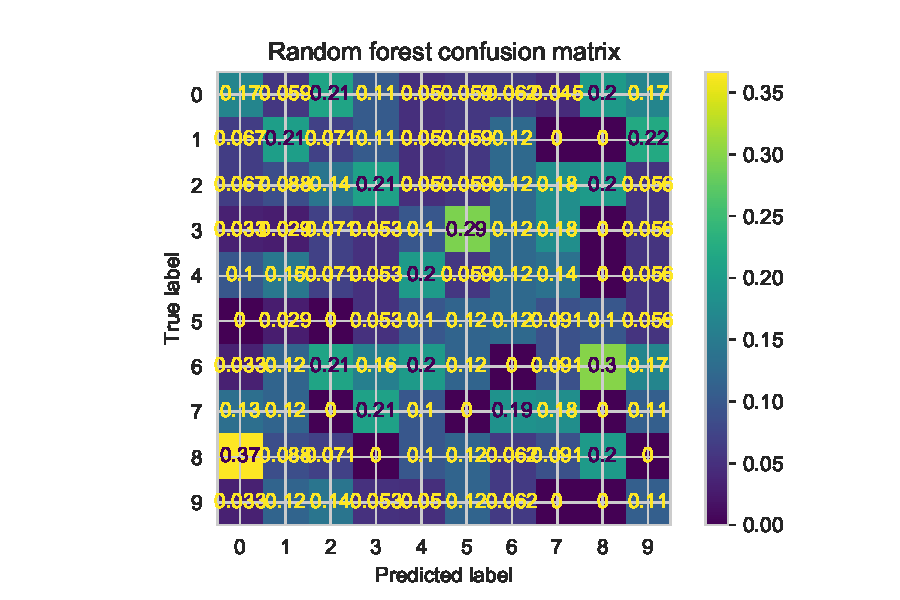
\includegraphics[width=1\linewidth]{figures/Tiny_Image/CM__Rndf_BOW.pdf}
\end{minipage}
\begin{minipage}[c]{0.5\textwidth}
\includegraphics[width=1\linewidth]{figures/Tiny_Image/CM__ppn_BOW.pdf}
\end{minipage}
\begin{minipage}[c]{0.5\textwidth}

\includegraphics[width=1\linewidth]{figures/Tiny_Image/CM__MLP_BOW.pdf}
\end{minipage}
\caption{Convusion matrices color histogram 1. Naive Bayes 2. Random Forest 3. Single Layer Perceptron 4. Multi Layer perceptron}
\label{CV_Matrices_Tiny_Image_BOW}
\end{figure}
%%%%%%%%%%%%%%%%%%%%%%%%%%%%%%%%%%%%%%%%%%%%%%%%%%%%%%%%%%%%%%%
\end{comment}


\section{Convolutional Neural Networks (CNN's)}
In this section we introduce the CNN architectures used for this work.

\subsection{SqueezeNet}
For the first architecture we decided on using SqueezeNet \cite{iandola2016}. SqueezeNet was developed with the goal to make it as compact as possible, but still achieving state of art results. In the original paper it is shown that SqueezeNet can achieve the same performance as an AlexNet for the ImageNet competition but with $50\times$ less parameters. This makes SqueezeNet particularly well suited for our small project where we need to rely on limited resources.

\subsection{Wrapped Res50Net for Transfer learning}
For the second architecture we have intensionally chosen a large one with many parameters, that gives the opportunity for transfer learning\footnote{\url{https://github.com/thushv89/manning_tf2_in_action/blob/master/Ch07/7.2.Transfer_Learning.ipynb}}. Here we aim to use Res50Net \cite{he2016deep}, which has over 23 Million trainable parameters. We wrap this architecture by a custom network and initialize it with the weights from the ImageNet competition. For the training we freeze all layers till layer 168 and train the remaining layers of Res50Net and the additional custom layers. More details are given in the results section.

\subsection{Training Details for CNN's}
For the training we are performing image augmentation and compare the obtained results to the case when no augmentation is applied. We apply for all CNN's the same random augmentations:
%
\begin{itemize}
	\item width/height shift up to $10\%$
	\item shearing up to $10\%$
	\item zoom up to $10\%$
	\item rotation up to $30^\circ$
	\item horizontal flip
\end{itemize}
%
For the training it was observed that the ADAM optimizer with learning rate $0.0001$ works well for all our cases. While performing the parameter search, we decrease the learning rate by a factor $0.1$, if the loss function did not decrease for the $5$ previous iterations, where the loss function is the categorial-crossentropy. Additionally if the loss function does not improve for $15$ iterations we stop the parameter search early. The parameter search is accelerated by a NVidia K80 GPU, but test-set evaluation times are measured when employing our CNN's on a Intel i5 CPU. Another important aspect is that we don't normalize the RGB scales of the pixels since this caused non-convergence for the most parameter searches. All CNN related analysis is performed as holdout, meaning we create a test, train validation set split. The reported objective that measures the quality of our predictions, while training the CNN is the accuracy that is defined as the number of correct predicted labels divided by the total number of samples we predict for a set. 



\subsection{Results Cifar10 Dataset}

\subsection{SqueezeNet}
For the Cifar10 Dataset the resulting SqueezeNet architecture has $740.554$ trainable parameters.
A holdout analysis is performed where we take $10\%$ of the train-data as validation data to evaluate the performance of the CNN at training time.

\begin{figure}
\centering
\SetFigLayout{3}{2}
  \subfigure[accuracy for SqueezeNet without augmentation]{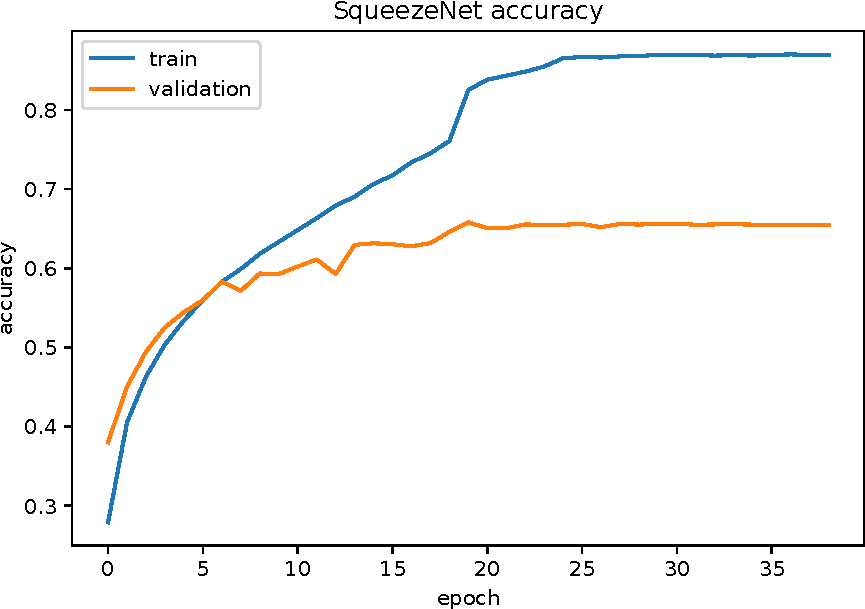
\includegraphics[width=0.45\columnwidth]{squeezeNet_cifar10_noaug.pdf}}
  \hfill
  \subfigure[accuracy for SqueezeNet with augmentation]{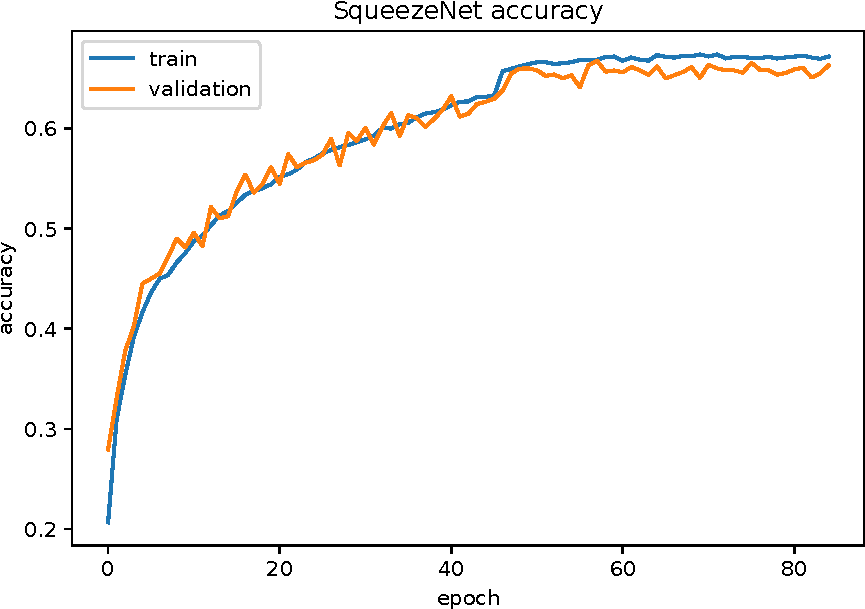
\includegraphics[width=0.45\columnwidth]{squeezeNet_cifar10_aug.pdf}}
  \hfill
\caption{Training-accuracy for SqueezeNet on the Cifar10 Dataset}
\label{rescnn::1}
\end{figure}

In figure \ref{rescnn::1} we can see the effect of the augmentation on the accuracy of the predictions while training. We have a clear overfitting of the CNN when not applying augmentation. This overfitting is largely decreased by applying the image-augmentation, as can be seen in the figure. When applying the augmentation, the accuracy of SqueezeNet on the test-set increased from $65.21\%$ to $67.33\%$. Augmentation of the images has an influence on the efficiency of the parameter search for the Network. Without augmentation the optimal parameters are found after $6 \min$ and less than $40$ epochs, whereas augmentation causes the time for parameter search to increase to $46 \min$ and $84$ epochs. For the prediction of the $313$ samples in the test-set SqueezeNet needs about $9 \text{s}$.

\begin{figure}
\centering
\SetFigLayout{3}{2}
  \subfigure[Confusion matrix for SqueezeNet trained on augmented Datase]{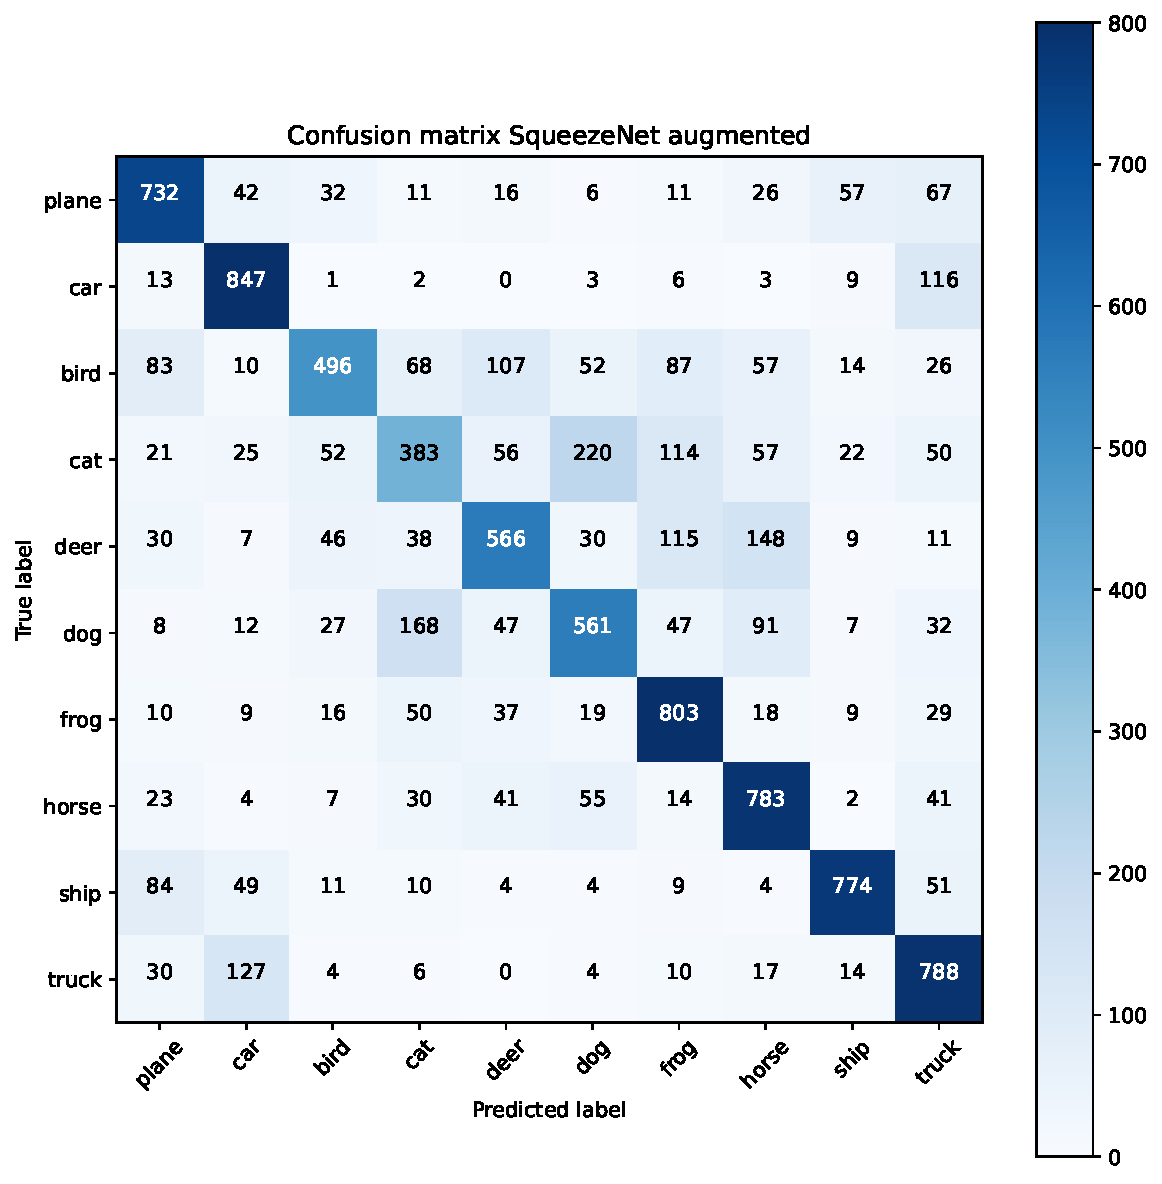
\includegraphics[width=0.45\columnwidth]{squeezeNet_cifar10_aug_confmat.pdf}}
  \hfill
  \subfigure[Confusion matrix for wrapped Res50Net trained on augmented Datase]{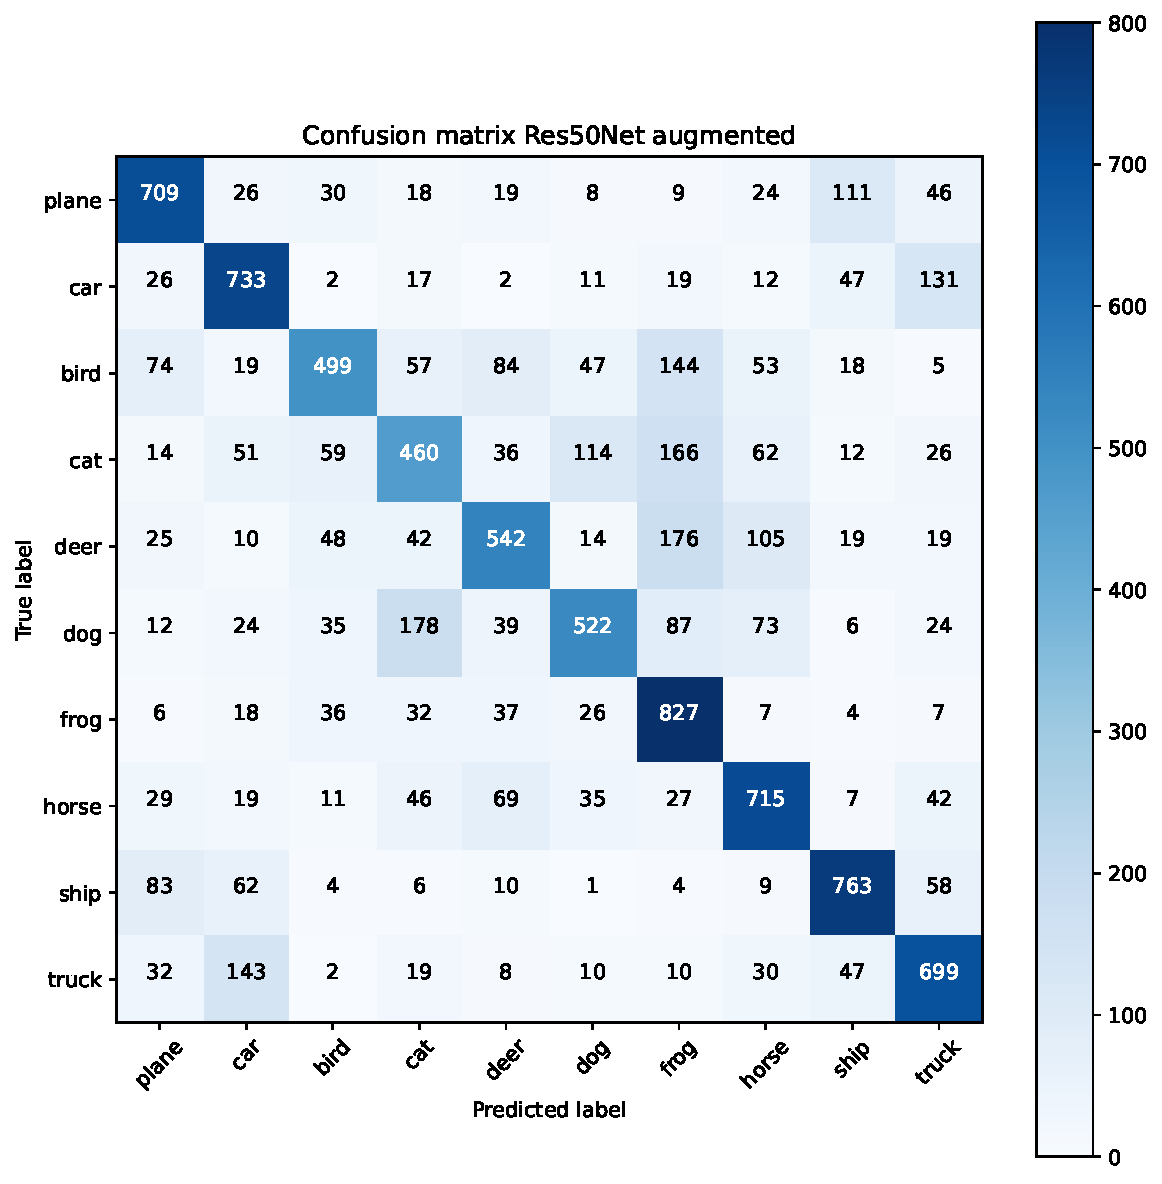
\includegraphics[width=0.45\columnwidth]{res50Net_cifar10_aug_confmat.pdf}}
  \hfill
\caption{Confusion Matrices of CNN architectures on the Cifar10 Dataset}
\label{rescnn::4}
\end{figure}

In figure \ref{rescnn::4} (a) we show the corresponding confusion matrix for the SqueezeNet trained on the augmented Cifar10 images. The most true positive labels are predicted for the car class, with $847$, where we note that $127$ times a truck sample gets confused to be a car. The least true positive labels are predicted for cats, with $383$, where this class often gets confused with the dog class. The most false negative predictions are made for the truck class with $423$ samples closely followed by the horse class with $421$ falsely predicted samples. This is due to the fact that trucks are often confused with cars and horses are often confused with deers or dogs.

\subsection{Res50Net}
To create our wrapped Res50Net, we stip off the top layers and replace that layer by a custom layer of $32\times 32 \times 3$ for reading our images. The output of the Res50Net gets fed into $3$ dense layers with $256, 128, 64$ neurons, till it reaches the softmax layers for prediction. Note that our dense layers consist each at the top of a batch normalisation layer and the dense layers with a dropout of $50\%$ for regularisation purposes. For the Res50Net layers in our CNN, we enable the training of the $168$ bottom layers and freeze the rest of them. By that we end up with a CNN that has in total $24.163.786$ parameters, from which are $3.986.762$ trainable. For the transfer learning we apply the same image augmentation as for SqueezeNet.

\begin{figure}
\centering
\SetFigLayout{3}{2}
  \subfigure[accuracy for Res50Net without augmentation]{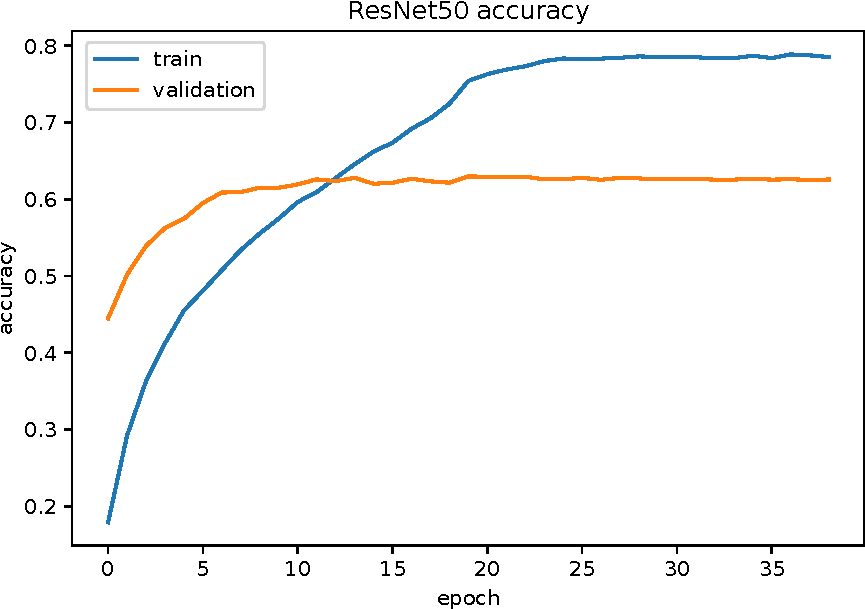
\includegraphics[width=0.45\columnwidth]{res50Net_cifar10_noaug.pdf}}
  \hfill
  \subfigure[accuracy for Res50Net with augmentation]{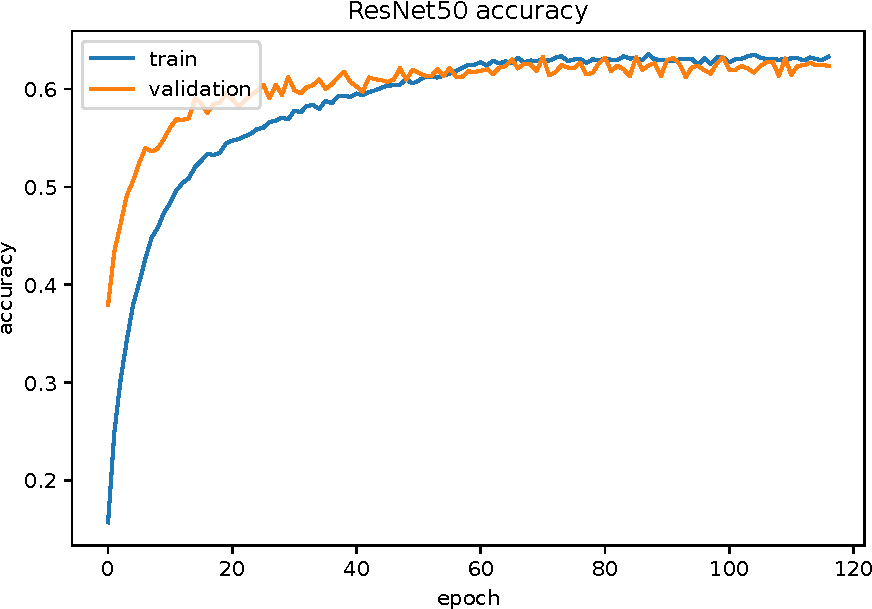
\includegraphics[width=0.45\columnwidth]{res50Net_cifar10_aug.pdf}}
  \hfill
\caption{Training-accuracy for Res50Net on the Cifar10 Dataset}
\label{rescnn::3}
\end{figure}

In figure \ref{rescnn::3} we show the accuracy while executing the transfer learning of Res50Net. Again without augmentation the CNN overfits till about $80\%$ accuracy on the trainset while the accuracy on the validation-set is $20\%$ lower. With augmentation we have diminished this effect and additionally improve the accuracy on the test-set from $62.16\%$ for no augmentation to $64.69\%$ with augmentation. The parameter-fitting for the augmented process took 117 epochs with a total time of $64 \min$ compared to that the parameter-fitting with no augmentation took $39$ epochs and about $10 \min$ in total. The evaluation on the test-set took $38\text{s}$ which is  $4$ times longer than for the SqueezeNet.

In figure \ref{rescnn::4} (b) the corresponding confusion matrix for the Res50Net trained on the augmented Cifar10 images is plotted. The most true positive predictions are made for the frog class with $827$. We also see that the frog class aswell has the most true negative predictions, where it seems particularly hard for the CNN to differentiate it from other animals. The cat class with the one with lowest true positives at $460$, where we note that $148$ dogs get wrongly classified as cats. Also notable is that cars get often confused as trucks and ships are often confused as planes.

\subsection{Results Tiny ImageNet Dataset}
\subsection{SqueezeNet}
On the Tiny ImageNet SqueezeNet has $838.024$ trainable parameters. First we plot in figure \ref{rescnn::5} the accuracy over the number of training epochs.

\begin{figure}
\centering
\SetFigLayout{3}{2}
  \subfigure[accuracy for SqueezeNet without augmentation]{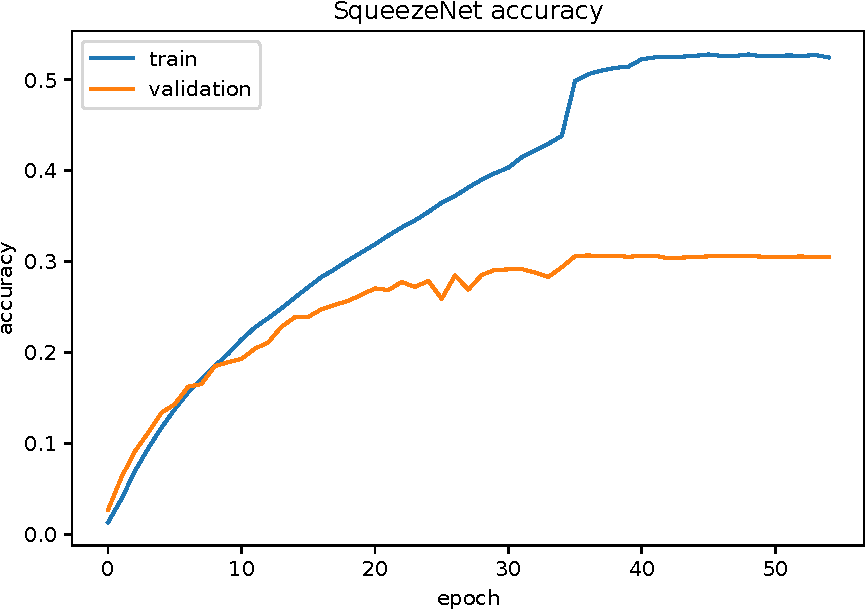
\includegraphics[width=0.45\columnwidth]{squeezeNetTIN_noaug.pdf}}
  \hfill
  \subfigure[accuracy for SqueezeNet with augmentation]{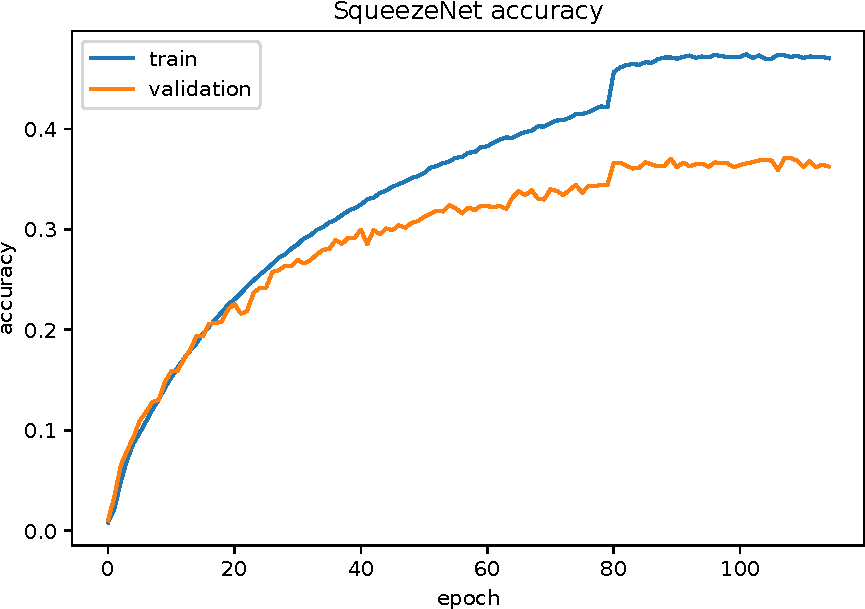
\includegraphics[width=0.45\columnwidth]{squeezeNetTIN_aug.pdf}}
  \hfill
\caption{Training-accuracy for SqueezeNet on the Tiny ImageNet Dataset}
\label{rescnn::5}
\end{figure}

As before we can examine less overfitting for the augmented case, but this time even with augmentation the SqueezeNet is overfitting as can be seen in the much higher accuracy of on the train-set compared to the accuracy on the validation-set. In both graphs we can identify the first decrease in learning rate by the jump in the training accuracy. Note that this jump occurs at a much later epoch for the augmented case showing more potential for improvement of the accuracy in the augmented case before reaching a local optimum. For the evaluation on the test-set, the SqueezeNet without augmented training-data has an accuracy of $31.26\%$ and augmentation caused the accuracy on the test-set to increase up to $34\%$. The tradeoff we pay is that for the training with no augmentation the parameter-search takes 55 epochs and $41 \min$, but with augmentation $115$ epochs and $297 \min$. Since the tiny ImageNet is larger than Cifar10 our evaluation time for SqueezeNet on the $10.000$ samples test-set is here about $60\text{s}$.

\begin{figure}
\centering
\SetFigLayout{3}{2}
\subfigure[confusion matrix of SqueezeNet with augmentation]{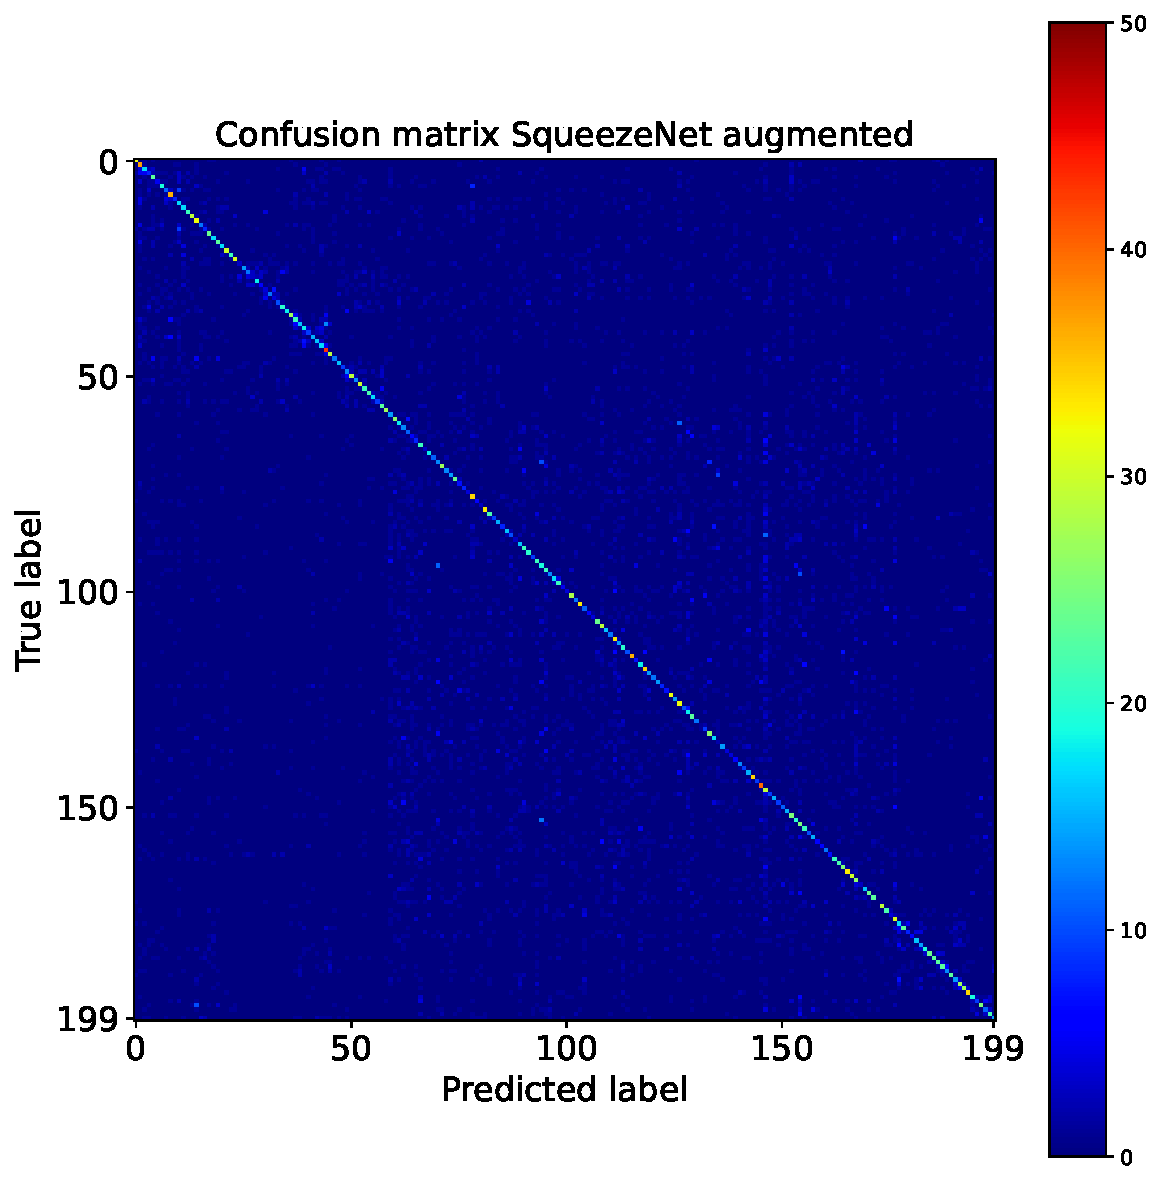
\includegraphics[width=0.45\columnwidth]{squeezeNet_TIN_aug_confmat.pdf}}
\hfill
\subfigure[confusion matrix of wrapped Res50Net with augmentation]{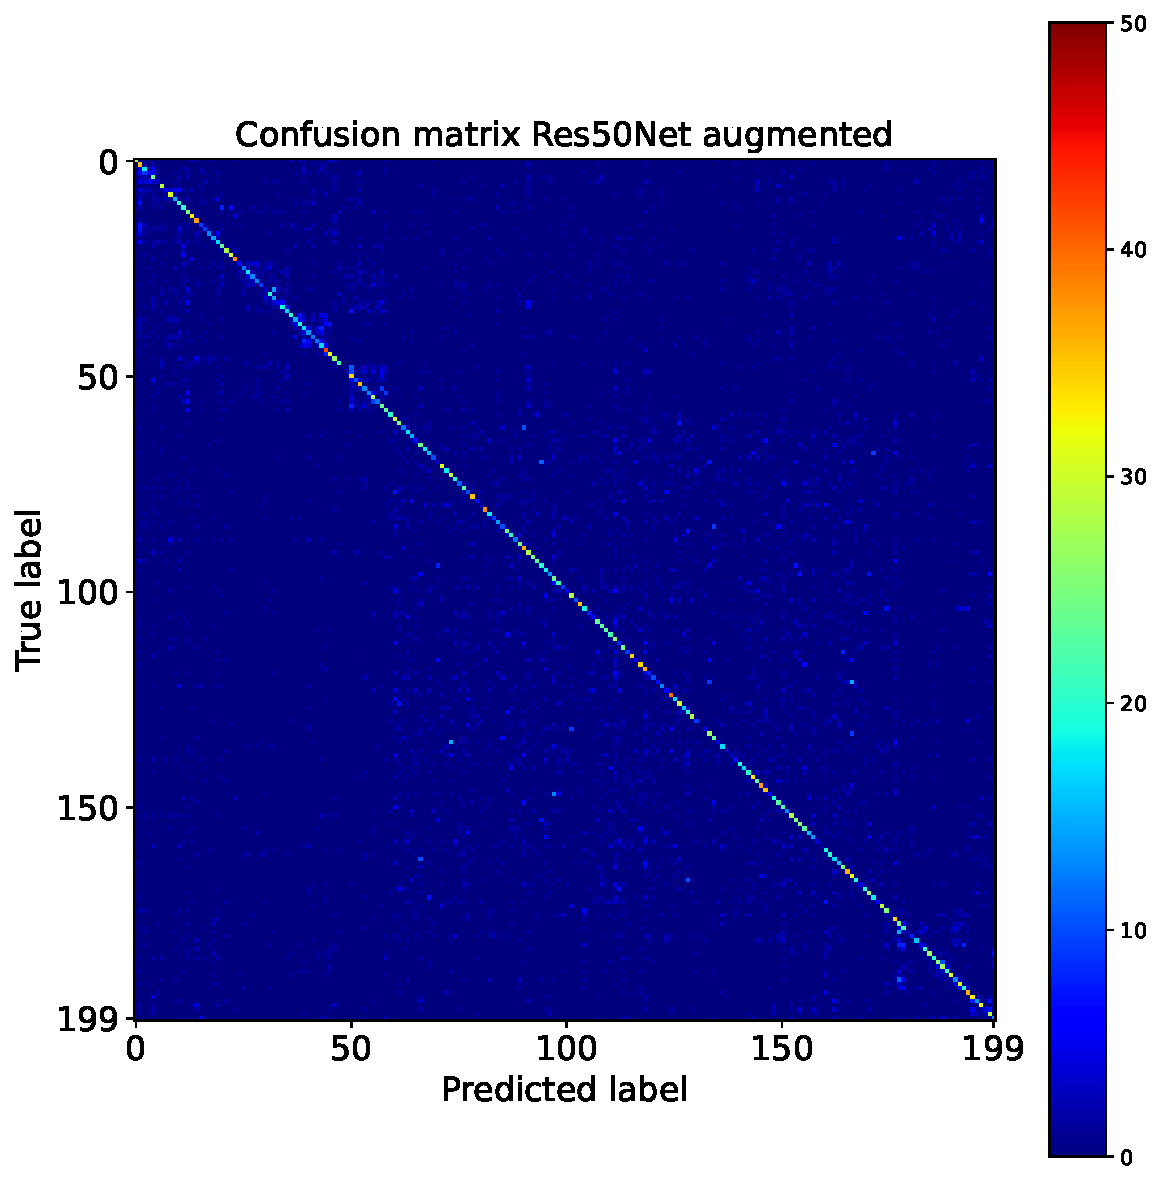
\includegraphics[width=0.45\columnwidth]{res50Net_TIN_aug_confmat.pdf}}
\hfill
\caption{Confusion matrices for CNN architectures on the augmented Tiny ImageNet Dataset.}
\label{rescnn::6}
\end{figure}

If we analyze the confusion matrix in figure \ref{rescnn::6} (a) we can measure the quality of our classifier by the size of the diagonal entries and the small off-diagonal entries.

Many classes have a large number of true positive predicted labels but to understand the classifier better analyze some special labels more closely. In table \ref{rescnn::7} is a summary of some important properties of the confusion matrix given.

\begin{table}[h]
\begin{tabular}{lc|lc|llc}
\toprule
             label &  corr. amount &                    label &  corr. amount & act. label &   pred. label &  times confused \\
\midrule
         water jug &               0 &                  monarch &              43 &          bee &           monarch &              13 \\
           plunger &               1 &               school bus &              40 &   sports car &       convertible &              12 \\
        pop bottle &               2 & fire salamander &              37 &    CD player &        scoreboard &              11 \\
            barrel &               3 &              black widow &              36 &        altar &             organ &              11 \\
          umbrella &               3 &                 lifeboat &              36 &  convertible &       beach wagon &              11 \\
Labrador  &               3 &                    brass &              34 &   coral reef &       brain coral &              10 \\
         Chihuahua &               3 &                 espresso &              34 &          dam & steel arch bridge &              10 \\
            bucket &               3 &               rugby ball &              34 &  beach wagon &       convertible &              10 \\
             chain &               3 &                  maypole &              34 &     scorpion &         centipede &               9 \\
          dumbbell &               4 &           triumphal arch &              33 &         slug &         centipede &               9 \\
\bottomrule
\end{tabular}
\caption{Some detailed information about the Confusion matrix of the SqueezeNet with augmented Tiny ImageNet }
\label{rescnn::7}
\end{table}

The first two columns state the classes that have the least amount of true positive predicted labels. Here we see that for the water jug we have no correct prediction whereas all other classes have at least one true positive predicted sample.For the classes with the highest number of correct predictions, we see in the next two columns that the monarch butterfly and secondly school busses were mostly correct identified. Further, we can state that often strong colored subjects are easily identified like school busses or life boats. In the last three columns the most confused labels are stated. Here we can extract that our SqueezeNet often confuses bees for monarchs or secondly sports cars as convertibles. This behaviour is as expected since ouch subjects are very closely related in shape and color.


\subsection{Res50Net}
For the Res50Net we again create a custom wrapper CNN where the input layer is defined for $64\times64\times 3$ images as required for Tiny ImageNet. The Res50Net's first 168 layers are not trained and we append additional three $256$ dense layers at the end where each has a batch normalisation layer at top and a dropout of $50\%$. The total parameters of the wrapped Res50Net are $25.902.920$ where $5.713.352$ are trainable.

\begin{figure}
\centering
\SetFigLayout{3}{2}
  \subfigure[accuracy for wrapped Res50Net without augmentation]{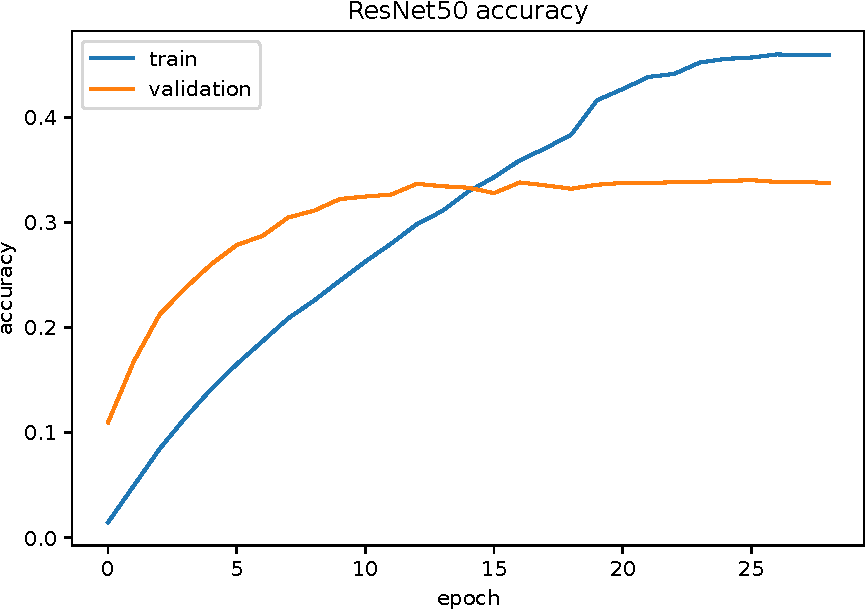
\includegraphics[width=0.45\columnwidth]{res50NetTIN_noaug.pdf}}
  \hfill
  \subfigure[accuracy for wrapped Res50Net with augmentation]{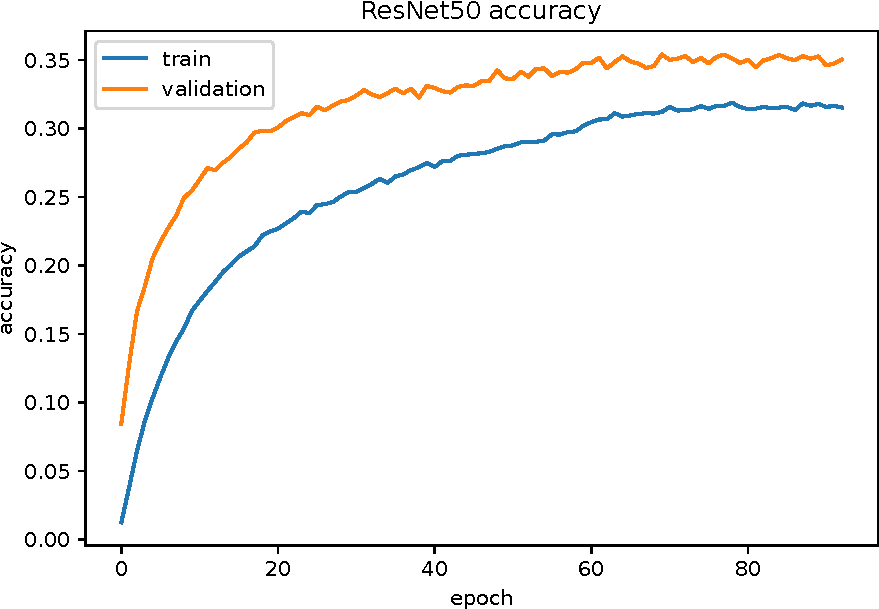
\includegraphics[width=0.45\columnwidth]{res50Net_TIN_aug.pdf}}
  \hfill
\caption{Training-accuracy for wrapped Res50Net on the Tiny ImageNet Dataset}
\label{rescnn::8}
\end{figure}

The training accuracies for the wrapped Res50Net are given in the two plots in figure \ref{rescnn::8}. For this case when using augmented images the accuracy on the validation-set is always higher than on the training-set in contrast to the studies before in this work. For the accuracy of the not augmented case on the test-set, we report $34.57\%$, where the running time was $42 \min$ with 39 epochs. For the augmented case we have a $37.7\%$ accuracy on the test-set, with a running time of $282\min$ over 93 epochs.For this architecture the prediction time for the $10.000$ test-samples is $103\text{s}$.

The confusion matrix for the augmented case is shown above in figure \ref{rescnn::6} (b). In the confusion matrix we can see that the network works well, since the off-diagonal entries are significantly lower than the diagonal ones for most of the columns. Again we cant do a in-depth analysis on such a large confusion matrix. Therefore, we extract some of the most important patterns from the confusion matrix and show them in table \ref{rescnn::9}.


\begin{table}[h]
\begin{tabular}{lc|lc|llc}
\toprule
       label &  corr. amount &              label &  corr. amount &   act. label & pred. label &  times confused \\
\midrule
     plunger &               0 &            monarch &              42 &     pop bottle &     beer bottle &              15 \\
         hog &               0 &            obelisk &              40 &      ice cream &           plate &              15 \\
     syringe &               1 &       bullet train &              38 &     moving van &      trolleybus &              15 \\
wooden spoon &               1 &             dugong &              38 &          tabby &    Egypt. cat &              14 \\
          ox &               2 &         school bus &              37 & sew. machine &            desk &              13 \\
      bucket &               2 &        brain coral &              37 &      meat loaf &           plate &              11 \\
  projectile &               2 &           espresso &              36 &    beach wagon &     convertible &              11 \\
   ice cream &               2 &     triumphal arch &              36 &            hog &           bison &              11 \\
       tabby &               3 &            maypole &              36 &         orange &           lemon &              10 \\
 beach wagon &               3 & Christ. stocking &              36 &      turnstile &       pay-phone &              10 \\
\bottomrule
\end{tabular}
\caption{Some detailed information about the Confusion matrix of the wrapped Res50Net with augmented Tiny ImageNet }
\label{rescnn::9}
\end{table}

When considering the first two columns in the table we see that the classes plunger and hog never get predicted correctly. All other classes have at least one correct prediction. Further, we see that without those $10$ classes with the least amount of correct predictions all other classes have already at least 3 correct predictions. Next when analysing the columns 3 and 4 in the table we see the classes that have the most correct predicted labels. Similar as in SqueezeNet the monarch, school bus and espresso are appearing here, which again suggests that large structures or objects with prominent colors can be recognized easier. Lastly when examining the 3 last columns on the right of the table we see the most confused classes. Mostly these confused classes describe objects that are very similar in shape and color like the pop bottle and beer bottle. But we see also that turnstiles are often confused with pay-phones, besides they are not too closely related. By that we see that the wrapped Res50Net CNN has still, potential for improvement and shortcomings like discussed could be improved by a more fine-grained training.


%Bibliography
\newpage
\bibliographystyle{plain}
\bibliography{lib}

\end{document}
